
\documentclass[a4paper,10pt,fleqn, twocolumn]{IEEETran}
\usepackage{amsfonts}
\usepackage{amsthm}
\usepackage{graphicx}
\usepackage{fancyhdr}



\setlength{\parindent}{3em} \setlength{\oddsidemargin}{0in}
\setlength{\textwidth}{6.5in} % sets 1in left and right margins
\setlength{\topmargin}{0.20in} % change to 0.2in for regular latex
%\setlength{\headheight}{0in}
%\setlength{\footheight}{0.5in}
\setlength{\footskip}{0.5in}
\setlength{\textheight}{9.0in} %sets 1in top and bottom margins
\renewcommand{\baselinestretch}{1} %set to 1.5 for double spacing.



\newcommand{\br}{{\mathbf r}}
\newcommand{\bA}{{\mathbf A}}
\newcommand{\ba}{{\bf a}}
\newcommand{\bb}{{\bf b}}
\newcommand{\bc}{{\bf c}}
\newcommand{\bC}{{\bf C}}
\newcommand{\bg}{{\bf g}}
\newcommand{\bG}{{\bf G}}
\newcommand{\bd}{{\bf d}}
\newcommand{\be}{{\bf e}}
\newcommand{\bs}{{\bf s}}
\newcommand{\bm}{{\bf m}}
\newcommand{\bn}{{\bf n}}
\newcommand{\bu}{{\bf u}}
\newcommand{\bv}{{\bf v}}
\newcommand{\bw}{{\bf w}}
\newcommand{\bx}{{\bf x}}
\newcommand{\by}{{\bf y}}
\newcommand{\bbf}{{\bf f}}
\newcommand{\bE}{{\bf E}}
\newcommand{\bF}{{\bf F}}
\newcommand{\bL}{{\bf L}}
\newcommand{\bM}{{\bf M}}
\newcommand{\bN}{{\bf N}}
\newcommand{\bS}{{\bf S}}
\newcommand{\bT}{{\bf T}}
\newcommand{\bD}{{\bf D}}
\newcommand{\bX}{{\bf X}}
\newcommand{\bP}{{\bf P}}
\newcommand{\bQ}{{\bf Q}}
\newcommand{\bI}{{\bf I}}
\newcommand{\bR}{{\bf R}}
\newcommand{\bU}{{\bf U}}
\newcommand{\bV}{{\bf V}}
\newcommand{\bW}{{\bf W}}
\newcommand{\bJ}{{\bf J}}
\newcommand{\bB}{{\bf B}}
\newcommand{\bzero}{{\bf 0}}
\newcommand{\bgamma}{{\mbox {\boldmath $\gamma$}}}
\newcommand{\btheta}{{\mbox {\boldmath $\theta$}}}
\newcommand{\bLambda}{{\mbox {\boldmath $\Lambda$}}}
\newcommand{\bPsi}{{\mbox {\boldmath $\Psi$}}}
\newcommand{\bPhi}{{\mbox {\boldmath $\Phi$}}}
\newcommand{\bcA}{{\mbox {\boldmath ${\cal A}$}}}
\newcommand{\bcB}{{\mbox {\boldmath ${\cal B}$}}}
\newcommand{\bcC}{{\mbox {\boldmath ${\cal C}$}}}
\newcommand{\bcD}{{\mbox {\boldmath ${\cal D}$}}}
\newcommand{\bcF}{{\mbox {\boldmath ${\cal F}$}}}
\newcommand{\bcN}{{\mbox {\boldmath ${\cal N}$}}}
\newcommand{\bcS}{{\mbox {\boldmath ${\cal S}$}}}
\newcommand{\bcH}{{\mbox {\boldmath ${\cal H}$}}}
\newcommand{\bcI}{{\mbox {\boldmath ${\cal I}$}}}
\newcommand{\bcR}{{\mbox {\boldmath ${\cal R}$}}}

\title{Blind Interference Cancellation}
\author{Shu Wang, Sang G. Kim, Li-Hsiang Sun, Hobin Kim,\\
   Suk W. Lee, S. R. Subramanya, Ki Y. Kim and Byung K. Yi\\ LGE Mobile Research (LGEMR), San Diego, CA 92131}
\date{}
\begin{document}
\maketitle
\begin{abstract}\small
In this paper, we propose several new blind multiuser detectors
for mitigating multiple access interference (MAI) and solving the
near-far problem in synchronous CDMA. These blind detectors are
developed with the ideas named as blind decorrelating, blind
multiuser signal model and linear prediction. Compared with
existing blind multiuser detectors, the proposed detectors require
a minimum number of previously received signals and no subspace
separation or channel/sequence estimation operation. Hence their
computation complexity can be much lower and detection delays are
much reduced. All these can be easily extended for asynchronous
CDMA. Theoretical analysis and computer simulations are provided
to demonstrate the performance of the proposed schemes.
\end{abstract}
\section{Introduction}
Multiuser detection strategy is a method for mitigating multiple
access interference (MAI) effects and solving the near-far problem
with exploiting interference structure~\cite{Verd98}. Recent
research has been devoted to blind multiuser detection and
subspace-based signature waveform estimation schemes for achieving
better performance and higher
capacity~\cite{Madh94,Honi95,Torl97,Wang98,Wang99,Zhang02}. Blind
multiuser detectors can achieve good performance with only the
knowledge of the timing and signature waveform of desired user(s).
This assumption also is much closer to practical applications.
There are two popular approaches for designing blind multiuser
detectors. One is to use the conventional multiuser signal
model~\cite{Verd98}, where received signals and multiuser
receivers are taken as linear combinations of actual spreading
sequences and noise, and statistical signal estimation techniques
for blind multiuser detection, e.g., the blind multiuser receiver
design using Wiener filters~\cite{Madh94,Honi95} or Kalman
filters~\cite{Zhang02} techniques. The other approach is based on
parametric signal modelling and signal spectrum estimation, where
received signals and multiuser receivers are taken as a linear
combination of desired users' spreading sequences and the
signal/noise subspace bases. Many subspace-based schemes are
examples of this approach, which essentially is an approach for
blindly reconstructing existing conventional multiuser detectors
using subspace concept~\cite{Wang98,Wang99}. One of the
difficulties in implementing the above approaches is that the
signal bases employed for designing blind multiuser receivers are
mostly unknown beforehand and it is nontrivial to accurately
estimate them. Therefore the required computation resources are
known to be too high for many practical applications, especially
when wireless channels and/or interfering signals experience fast
dynamic change.

In order to solve the near-far problem with minimum prior
knowledge and computation complexity, we propose a new blind
multiuser framework based on a blind multiuser signal model in
this paper. This blind signal model is different from the
traditional linear prediction model~\cite{Haykin96}~\footnote{The
discussion of the relationship between linear prediction model and
the proposed framework is omitted because of the length limitation
of this paper. It will be addressed in another paper.} and the
widely-discussed conventional signal model and subspace-based
parametric signal model. In the proposed model, each received
signal can be taken as a linear combination of desired users'
spreading sequences, several previously received signals and/or
noise. Based on this new blind multiuser signal model and
detection framework, several blind multiuser detectors are
developed using BLU and MMSE estimation criteria in addition to
the LS-based schemes in~\cite{Wang03d,Wang03e}. The proposed
algorithms are simple and direct only using the signatures and
timing of desired users. There is no converging, estimation or
subspace separation procedure employed by many other blind
detectors~\cite{Madh94,Honi95,Wang98,Wang99}. Compared with
existing blind detection schemes, they require a minimum number of
previously received signals. Hence the computation complexity and
detection delay can be much reduced. A recursively adaptive
implementation is also provided to further lessen the required
computation complexity. Theoretical analysis and computer
simulations are finally presented to demonstrate the performance
of these blind detectors.
\section{System Model And Problem Description}
We consider forward-link transmissions in a single-cell DS/CDMA
system. There are $K$ active users over the multipath channel with
$P$ strong paths~\footnote{Strong paths are those to be explicitly
combined by RAKE receiver.} and the channel is an additive white
Gaussian noise (AWGN) channel. The baseband representation of the
received signal due to user $k$ is given by
\begin{equation}
\begin{array}{rcl}
r_k(t)&=&\sum\limits_{p=1}^{P}\alpha_{pk}A_k[n]
b_k[n]c_k(t-nT-\tau_p)
\end{array}
\end{equation}
\noindent where $\alpha_{pk}$ is the $p$th path loss of user $k$'s
signal, $b_k{[n]}$ is the $n$th bit sent by user $k$. We assume
that the $\left\{b_k{[n]}\right\}$ are independent and identically
distributed random variables with $E\left\{b_k{[i]}\right\}=0$ and
$E\left\{|b_k{[i]}|^2\right\}=1$. The parameters $c_k(t)$ denote
the normalized spreading signal waveform of user $k$ during the
interval $[0,\ T]$, $\tau_1\leq\tau_2\leq\ldots\leq\tau_P$,
denotes $P$ different transmission delays from the base station to
user $k$ and $A_k[n]$ is the amplitude of the received signal for
user $k$ at time $t=n$. The total baseband signal received by user
$k$ is
\begin{equation}
\begin{array}{rcl}
\tilde{r}(t)&=&\sum\limits_{k=1}^{K}r_k(t)
\end{array}
\end{equation}
The received signal $\tilde{r}(t)$ is passed through the
corresponding chip matched filter (CMF) $\phi(t)$ and RAKE
combiner. The combined output $r(t)$ is~\footnote{Without loss of
the generality, we drop the time index $n$ in the following
discussion.}
\begin{equation}\hspace{-0.0in}
\begin{array}{rcl}
r(t)&=&A_k b_k c_k(t-nT-\tau_1)\otimes \phi(t-\tau_1)+ \\
&&\hspace{0.0in} m_{\rm ISI}(t) + m_{\rm MAI}(t) + n(t)
\end{array}\label{r_t}
\end{equation}
\noindent where
\begin{equation} \hspace{-0.05in}
\begin{array}{rcl}
 m_{\rm ISI}(t)&=&\\
 &&\hspace{-0.83in}\sum\limits^{P}_{p\neq
q}\beta_{qk} \alpha_{pk}A_kb_kc_k(t-nT+\tau_{q1}-\tau_1)\otimes
\phi(t-\tau_1)
\end{array}
\end{equation}
\noindent is the intersymbol interference (ISI) to user $k$,
\begin{equation} \hspace{-0.17in}
\begin{array}{rcl}
m_{\rm MAI}(t)&=&\sum\limits_{i\neq
 k}^{K}A_ib_ic_i(t-nT-\tau_1)\otimes\phi(t-\tau_1)+\\
 &&\hspace{-0.75in}\sum\limits_{i\neq
 k}^{K}\sum\limits^{P}_{p\neq
q}\beta_{qk}
\alpha_{pi}A_ib_ic_i(t-nT+\tau_{q1}-\tau_p)\otimes\phi(t-\tau_1)
\end{array}
\end{equation}
\noindent is the MAI to user $k$, $\beta_{qk}$ is the weight of
the $q$th RAKE finger with
$\sum\limits_{q=1}^{P}\beta_{qk}\alpha_{qk}=1$ and $\tau_{q1} =
\tau_{q}-\tau_1$ is the propagation delay difference between the
$1$st path and $p$th path. $\otimes$ denotes the convolutional
product. $n(t)$ is AWGN with variance $\sigma^2$. The user $k$'s
RAKE output can be sampled at $f_s=1/T_s$ and straightforwardly
expressed by
\begin{equation}\hspace{-0.1in}
\begin{array}{rcl}
\br&=&\left[
\matrix{r(nT+T_s+\tau_1)&\ldots&r(nT+LT_s+\tau_1)}\right]^{\rm
T}\\
 &=&\sum\limits_{k=1}^{K} A_k b_k \bs_k + \bn \\
 &=&\bS \bA \bb + \bn
\end{array}\label{r_sync}
\end{equation}
\noindent where $\bS=[\bs_1\ \bs_2\ \ldots\ \bs_K]$ is the
received spreading sequence matrix combined with both ISI and MAI
information, and $L=T/T_s$ is the number of samples per symbol,
which should not be less than the spreading gain $L_c$.

Because of $m_{\rm MAI}(t)$ existing in the received signal
$r(t)$, the performance of conventional matched filter receiver
suffers from the so-called near-far problem~\cite{Verd98}.
Multiuser detection is the receiver technique for solving this
problem and most multiuser detectors are firstly developed using
the conventional system model like (\ref{r_sync}). These are well
documented in~\cite{Verd98}. One of the difficulties in developing
blind multiuser detectors using (\ref{r_sync}) is that the $\bS$
is hard to be known beforehand. And it normally takes much effort
to determine it later. The similar situation can also be met in
developing blind detectors using the parametric subspace signal
model proposed in~\cite{Wang98}.
\section{Direct Blind Multiuser Detections}

\subsection{Blind Decorrelating Detection}

\subsection{Blind Multiuser Detection Using Linear Prediction}

\subsection{Blind Multiuser Signal Model and Multiuser Detection Framework}
\begin{figure} \center{
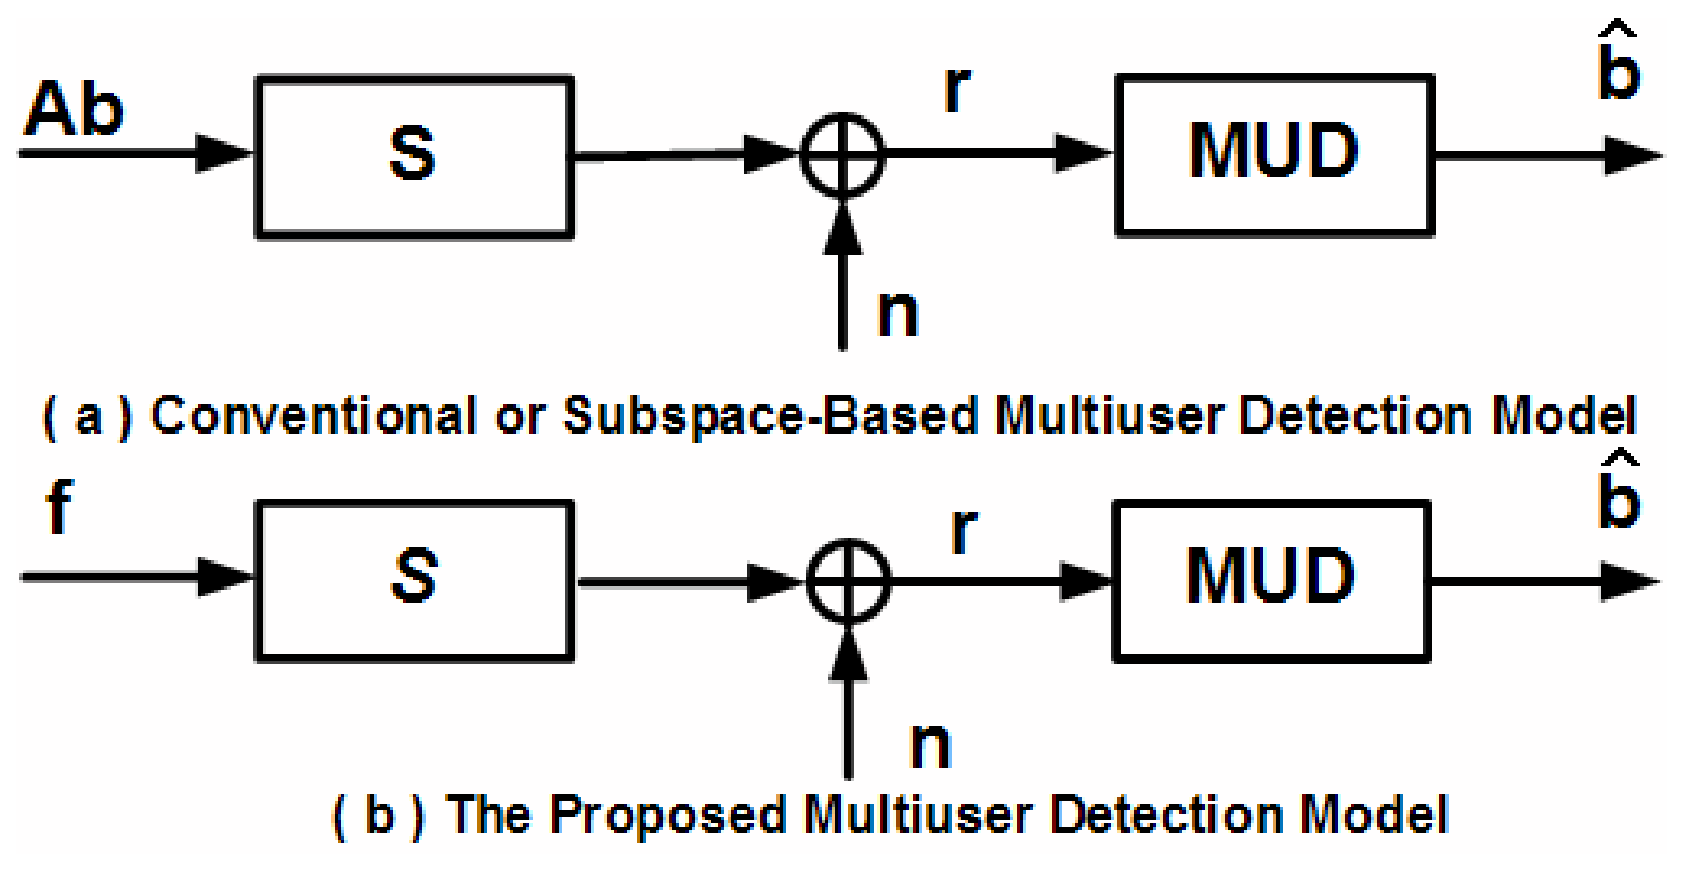
\includegraphics[width=3in]{MUD_model.eps}
\caption{Multiuser detection models.  } }\label{MUD_model}
\end{figure}
Instead of using the conventional signal model or the parametric
subspace signal model, we develop a new blind multiuser signal
model shown in Fig. 1, which uses a blind but "faked" spreading
matrix $\bcS$ for desired user(s). We call $\bcS$ the blind but
"faked" spreading matrix because 1) it is composed by only desired
users' spreading sequences and previously received signals and 2)
it isn't the original one but works like the original one. Without
loss of the generality, only the bits sent for first $G$ users are
considered here and the $L\times M$ blind spreading sequence
matrix $\bcS$ is defined by
\begin{equation}
\begin{array}{rcl}
\bcS&=&[\matrix{\bs_1&\ldots&\bs_G&{\br}_{1}&{\br}_{2}&\ldots&{\br}_{M-G}}]\\
\end{array} \label{S_0}
\end{equation}
\noindent where $\bs_g$, $g=1,\ 2,\ \ldots,\ G$, denote the group
of $G$ spreading waveforms which are already known to user $1$.
${\br}_m$, $m=1,\ 2,\ \ldots,\ M-G$, are $M-G$ previously received
independent signal vectors~\footnote{The first $M-G$ received
signal $\br_m$ may be obtained from some receiver initialization
procedure. After that, there will be some possible adaptive
procedure for updating $\bcS$, e.g. the procedure proposed in
Section \ref{updatingG}. Compared with existing blind detectors,
this number, $M-G$, of required previously received signals are
very small.}. $K\leq M\leq L$. Obviously $M=K$ is the minimum
number for blind multiuser detector to unambiguously distinguish
different interfering signals. And if $M>L$, blind multiuser
receiver will not be unique since there will be more variables
than available equations. The relationship between the proposed
blind spreading matrix $\bcS$ and the original spreading matrix
$\bS$ can be given by
\begin{equation}
\begin{array}{rcl}
\bcS &=&\bS\bB + {\bN}\\
\end{array}\label{S_1}
\end{equation}
\noindent where the first $G$ columns of $\bcS$ and $\bS$ are
same,
\begin{equation}\hspace{-0.0in}
\begin{array}{c}
 \bB=\left[\matrix{\bI & \bar\bD\cr\bzero&\tilde\bD }\right]=\left[\matrix{\bE & \matrix{\bar\bD\cr \tilde{\bD}} }\right]
  =\left[\matrix{\bG \cr \matrix{\mathbf{0}& \tilde{\bD}}
 }\right]
\end{array}\label{B}
\end{equation}
\noindent is the $K\times M$ data matrix associated with $\bcS$.
$\bE=[\matrix{\bI&\bzero}]^{\rm T}$, $\bG = \left[\matrix{\bI&
\bar\bD}\right]$ is the $G\times M$ matrix composed by known data
in $\bcS$. $\mbox{rank}\{\tilde{\bD}\}=K-G$ and
$\mbox{rank}\{\bB\}\leq K$. Combining (\ref{r_sync}) and
(\ref{S_0}), the received signal vector $\br$ in (\ref{r_sync})
can be expressed as the linear combination of the columns in
$\bcS$ instead of $\bS$, which is written by
\begin{equation}
\begin{array}{rcl}
\br&=&\bcS\bbf + \bar{\bn} \label{r_blind}
\end{array}
\end{equation}
\noindent where the $M \times 1$ vector $\bbf$ is termed the
detection vector defined by
\begin{equation}
\begin{array}{rcl}
\bbf&=&\bB^{+}\bar\bb
\end{array} \label{DetectorVector}
\end{equation}
\noindent where $[\cdot]^{+} $ denotes the general inverse
operator and $\bar\bb=\bA \bb$. $\bar{\bn}$ is the new $L\times 1$
noise vector defined by
\begin{equation}
\begin{array}{rcl}
\bar{\bn}&=&\bn-{\bN}\bB^{+}\bar\bb
\end{array} \label{new_noise}
\end{equation}
We can see that (\ref{r_blind}) may be taken as a modified linear
prediction model and the multiuser detection problem may be taken
a modified linear prediction problem~\footnote{Blind multiuser
detection using linear prediction will be discussed in another
paper.} if $\bar{\bn}=\bzero$. On the other hand, if $\bbf$ can be
estimated, the amplitudes $A_g$ and bits $b_g$ for the first $G$
users can be estimated and detected with (\ref{DetectorVector}) by
\begin{equation}\hspace{0.2in}
\begin{array}{l}
\hat{\bb}_1
=\left[\matrix{\hat{b}_1&\hat{b}_2&\ldots&\hat{b}_G}\right]^{\rm
T}=\mbox{sgn}\left\{\bG\bbf\right\}\
\end{array}, \label{b_estimation}
\end{equation}
\begin{equation}\hspace{-0.40in}
\begin{array}{l}
\hat{\ba}_1
=\left[\matrix{\hat{A}_1&\hat{A}_2&\ldots&\hat{A}_G}\right]^{\rm
T}=\left|\bG\bbf\right|\ .
\end{array} \label{A_estimation}
\end{equation}

In the following, we will present various schemes for estimating
$\bbf$ and detecting $\bb_1$. An adaptive implementation will be
presented in Section \ref{updatingG}.
\section{Adaptive Implementation\label{updatingG}}
\begin{figure}
\center{
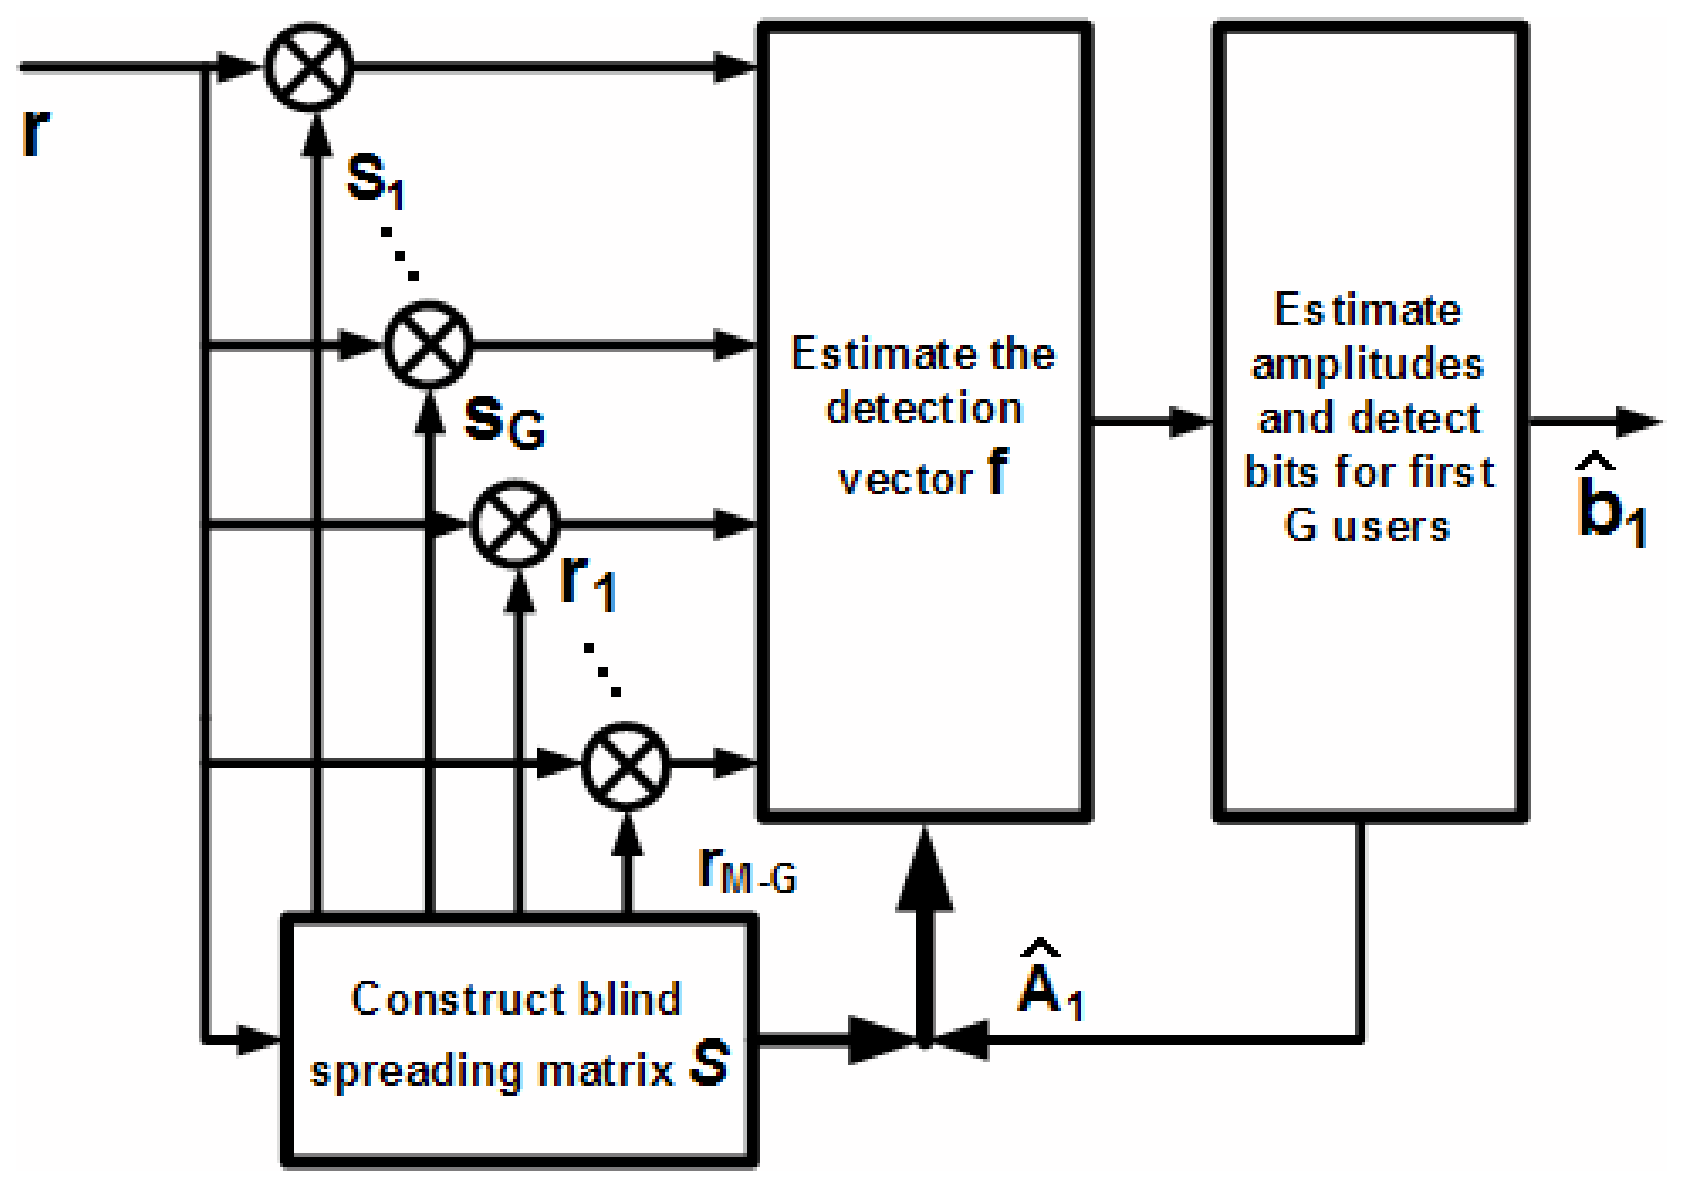
\includegraphics[width=2.5in]{BMUD_structure12.eps}
\caption{ The proposed adaptive blind multiuser detection
structure.} }\label{AMUDstruct}
\end{figure}
In Fig. 2, an adaptive structure of the presented blind multiuser
detection scheme is presented for time-variant channels. Following
the well-known Sherman-Morrison-Woodbury matrix inverse
lemma~\cite{Haykin96,Golu96}, a recursively adaptive
implementation of the proposed LS and BLU blind detector can be
expressed by
\begin{equation}\hspace{-0.0in}
\begin{array}{rcl}
\hat{\bb}_1(n)&=&\mbox{sign}\left\{\bG(n)\bcC_{\cal
S}^{+}(n)\bcS^{\rm T}(n)\br(n)\right\}
\end{array}
\end{equation}
\begin{equation}\hspace{-0.0in}
\begin{array}{l}
\bcC_{\cal S}^{+}(n)=\bcC_{\cal S}^{+}(n-1)-\frac{\bcC_{\cal
S}^{+}(n-1)\bu(n-1)\bu^{\rm T}(n-1)\bcC_{\cal
S}^{+}(n-1)}{1+\bu^{\rm T}(n-1)\bcC_{\cal S}^{+}(n-1)\bu(n-1)}
\end{array}\label{adaptiveLS}
\end{equation}
\noindent where
\begin{equation}\hspace{-0.0in}
\begin{array}{rcl}
\bcC_{\cal S}(n)&=&\bcS(n)^{\rm T}\bcS(n)
\end{array}
\end{equation}
 \noindent and $\bu(n-1)$ is designed using SVD so that
\begin{equation}\hspace{-0.00in}
\begin{array}{rcl}
\bu(n-1)\bu^{\rm T}(n-1)&=&\bcC_{\cal S}(n)-\bcC_{\cal S}(n-1)
\end{array}
\end{equation}
\section{Performance Analysis}
\subsection{AME and Near-Far Resistance}
A commonly used performance measure for a multiuser detector is
asymptotic multiuser efficiency (AME) and near-far
resistance~\cite{Verd98}. Since the proposed algorithms converges
to the conventional decorrelating detector as $\sigma^2\rightarrow
0$, their AME and near-far resistance are identical to the
decorrelating detector:
\begin{equation}
\begin{array}{rcl}
\bar{\eta}_k&=&\frac{1}{\bR_{kk}^{+}}
\end{array}.
\end{equation}
\subsection{CRLB for $\bbf$ Estimation}
The Cram\'{e}r-Rao Lower Bound (CRLB) is given by the inverse of
the Fisher information matrix (FIM). Providing the blind spreading
matrix $\bcS$ is known beforehand, we first define the parameter
vector $\mathbf{\phi} = \left[\bar{\sigma}^{2}\ \bbf^{\rm
T}\right]^{\rm T}$, where $\bar{\sigma}^{2}
=(1+\frac{M-G}{M-K})\sigma^{2}$, for computing the FIM
\begin{equation}
\begin{array}{rcl}
{\bI(\mathbf{\phi})} &=& {\rm E} \left\{ \left( \frac{\partial
\ln{\cal L}}{\partial \mathbf{\phi}} \right) \left( \frac{\partial
\ln{\cal L}}{\partial \mathbf{\phi}} \right)^{\rm H} \right\}
\label{fim}
\end{array}
\end{equation}
\noindent where $\ln{\cal L}$ is the log-likelihood function given
by
\begin{equation}
\begin{array}{rcl}
\ln{\cal
L}&=&C-L\ln\bar{\sigma}^2-\frac{1}{2\bar{\sigma}^2}\parallel\mathbf{e}\parallel_2^2
\end{array},\label{logl}
\end{equation}
\noindent $C$ is a constant and $\mathbf{e}=\br-\bcS\bbf$.
Providing $\bcS$ is known, the closed-form CRLB expression of
$\bbf$ is then given by
\begin{equation}
\begin{array}{rcl}
{\rm CRLB}(\bbf\ |\ \bcS) &
=&(1+\frac{M-G}{M-K})\sigma^{2}(\bcS^{\rm T}\bcS)^{\rm +}
\end{array}.\label{CRLB_f}
\end{equation}
\noindent It shows that the accuracy of estimating $\bbf$ may
increase with increasing $M$.
\section{Computer Simulations}
There are $K=10$ users with the group size $G=3$ and the spreading
sequences used in simulations are $64$-chip ($L=64$) random
sequences. In the computer simulations, the previous amplitude
estimation from (\ref{A_estimation}) is directly use for the next
detection without any amplitude filtering. From Subplot (a) in
Fig. 3, it is interesting to see that the performance of the
simplest LS detector has the best performance. From Subplot (b),
it is very impressive to find that the performance of blind LS
detector is very close to the conventional decorrelating detector
whatever how strong the MAI is in our simulations when $M$ is
large enough. We then check the performance of the proposed LS
blind detector against the amplitude estimation errors. From Fig.
4, we can see that the BER of the LS detector basically is
unchanged against amplitude estimation error when SNR is large
enough. From Fig. 5, we can see that the performance of the LS
detector can be better providing $M$ is larger enough. This
confirms (\ref{noise_var_new}), which shows that the variance of
$\bar{\bn}$ decrease with increasing $M$.
\begin{figure} \center{
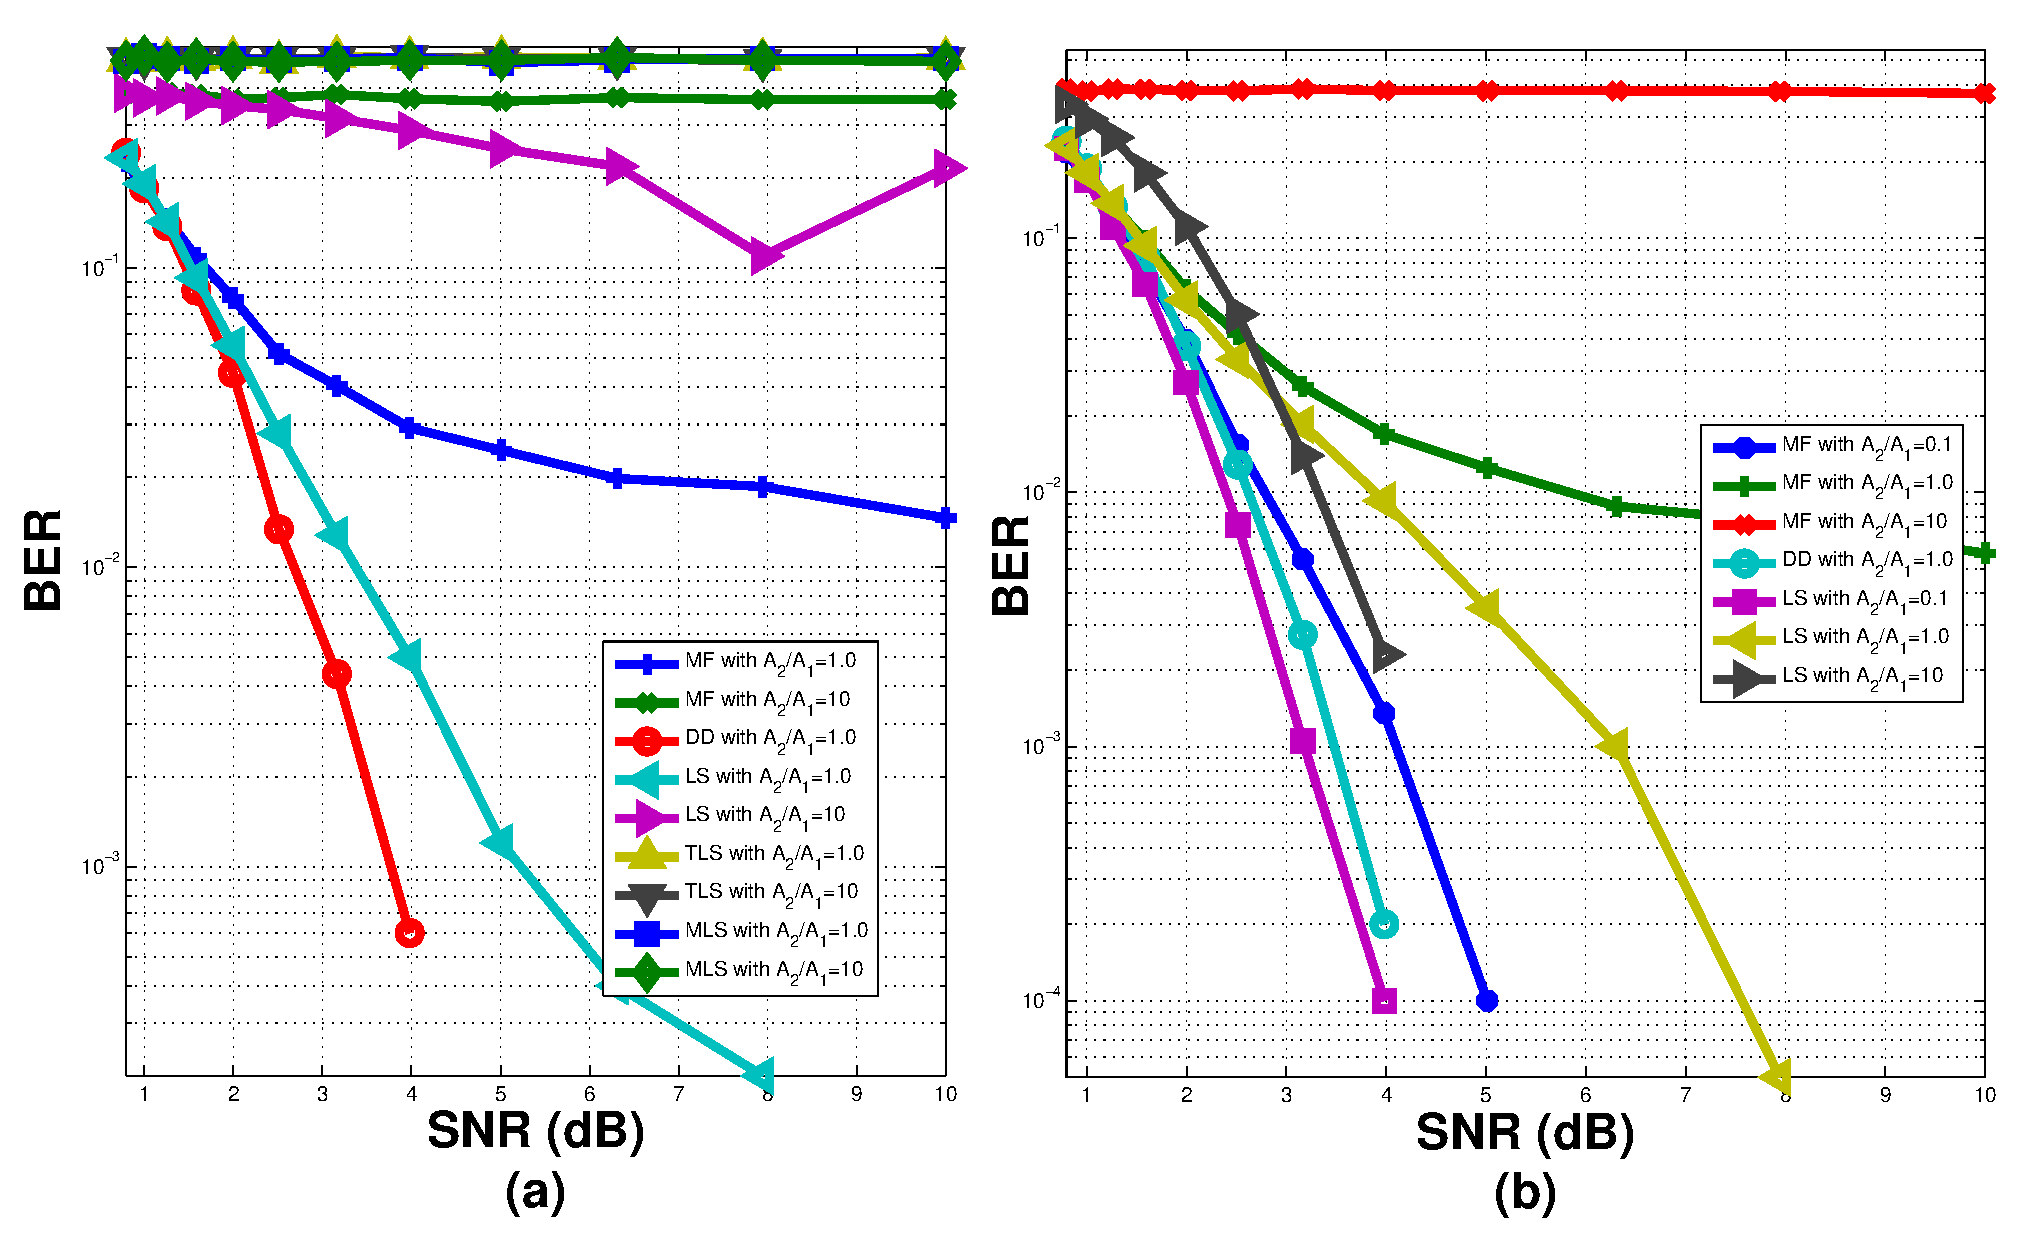
\includegraphics[width=3in]{BER_SNR_10_64.eps}
\caption{ (a) The performance of the proposed blind MUDs against
SNR, $M=12$. (b) The performance of the proposed blind LS
detector, $M=63$. } }\label{BER_SNR}
\end{figure}
\begin{figure} \center{
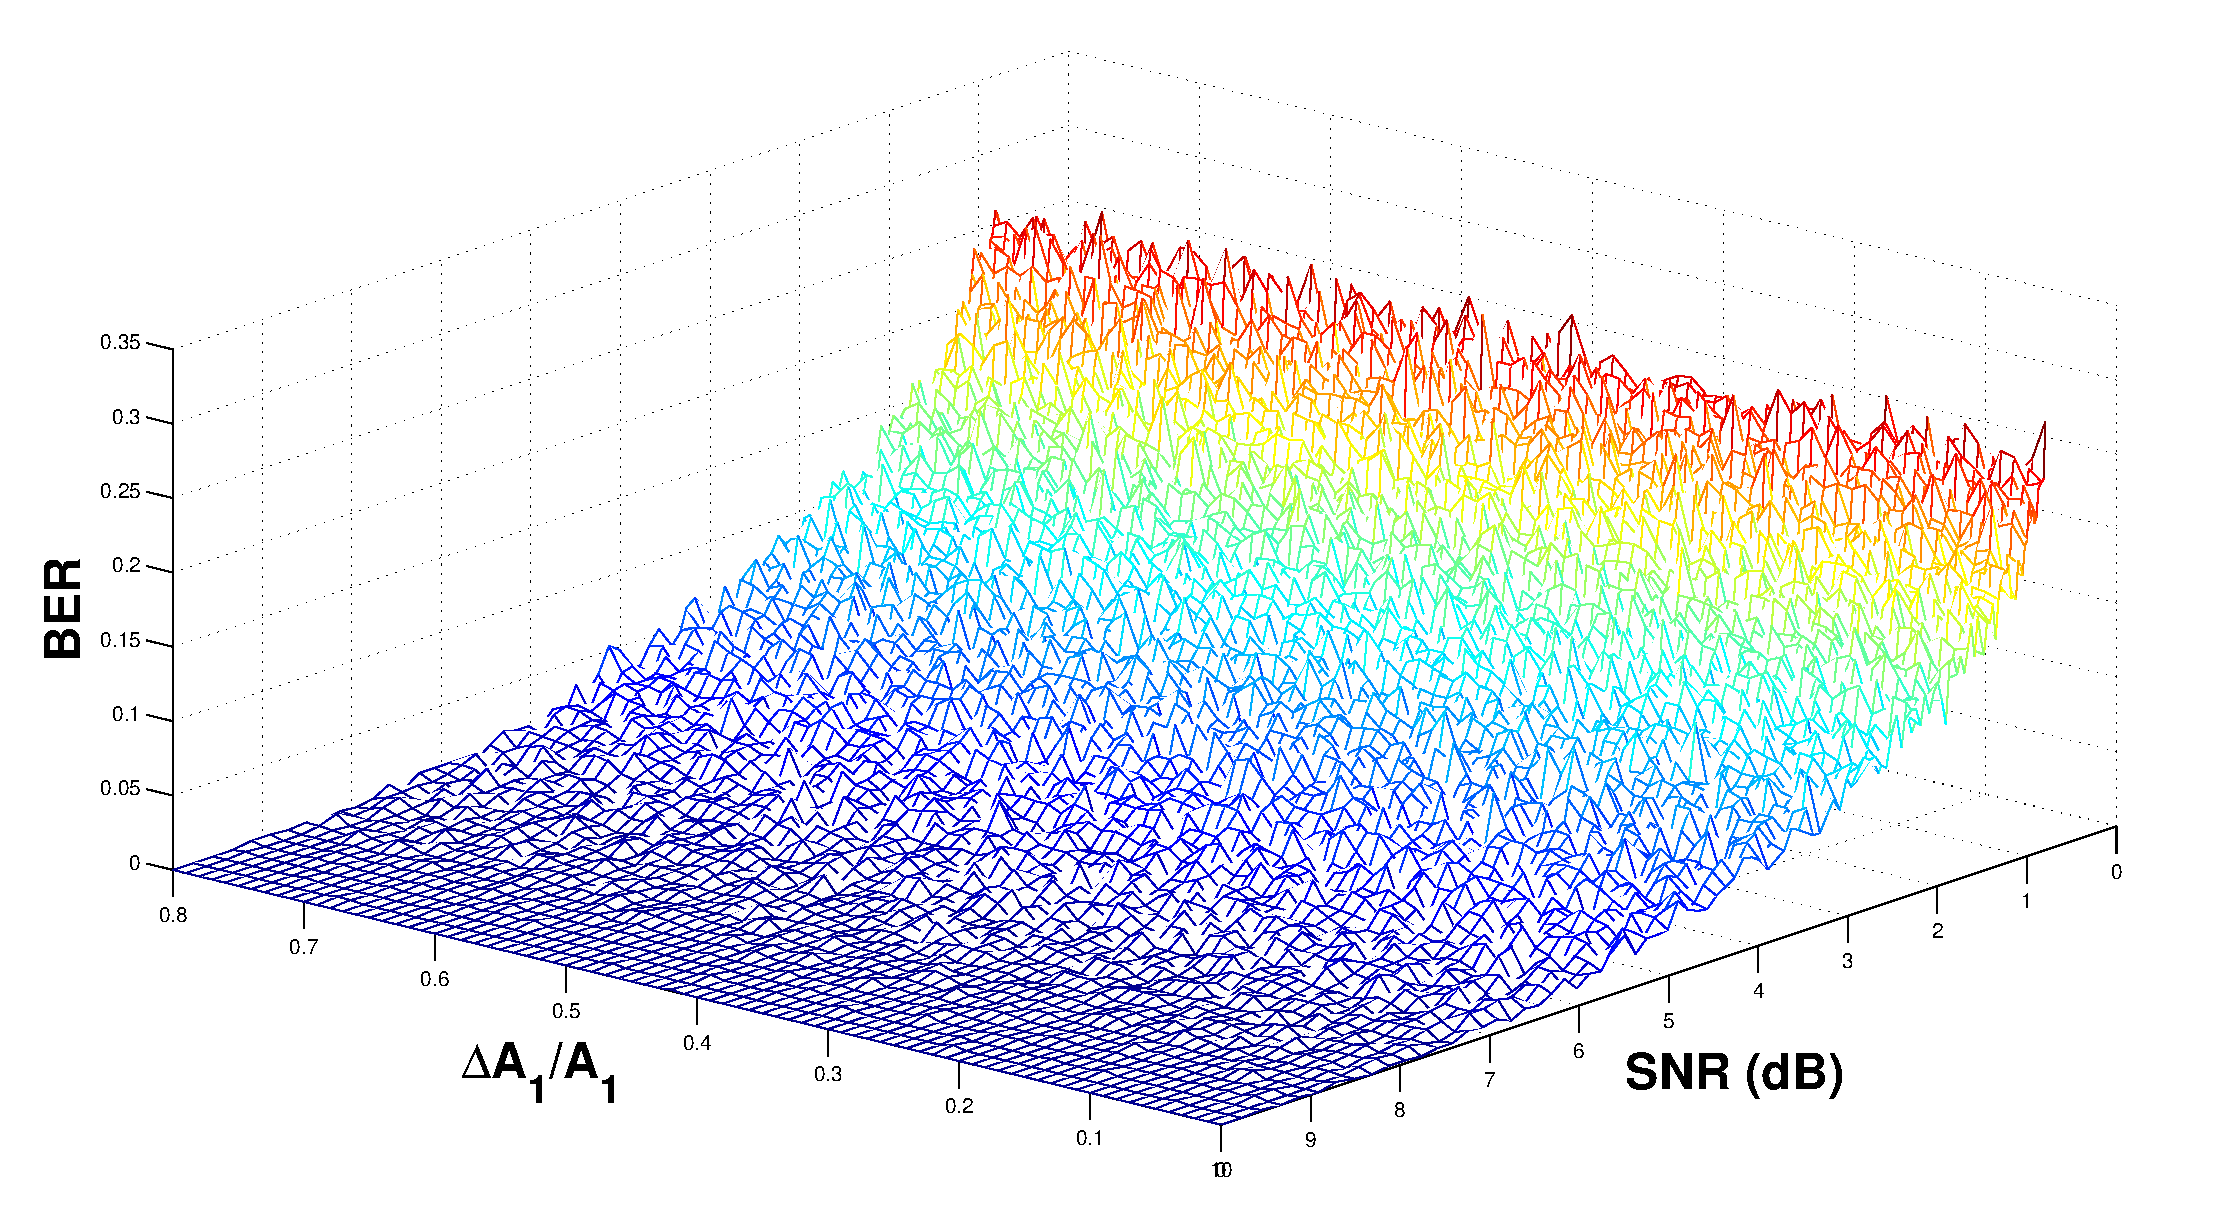
\includegraphics[width=2.5in]{BER_A_SNR_10_64_LSs.eps}
\caption{ The performance of the LS detector against amplitude
estimation error ${\Delta}{A_1}/A_1$ and SNR, $M=63$.}
}\label{BER_A_SNR}
\end{figure}
\begin{figure}
\center{
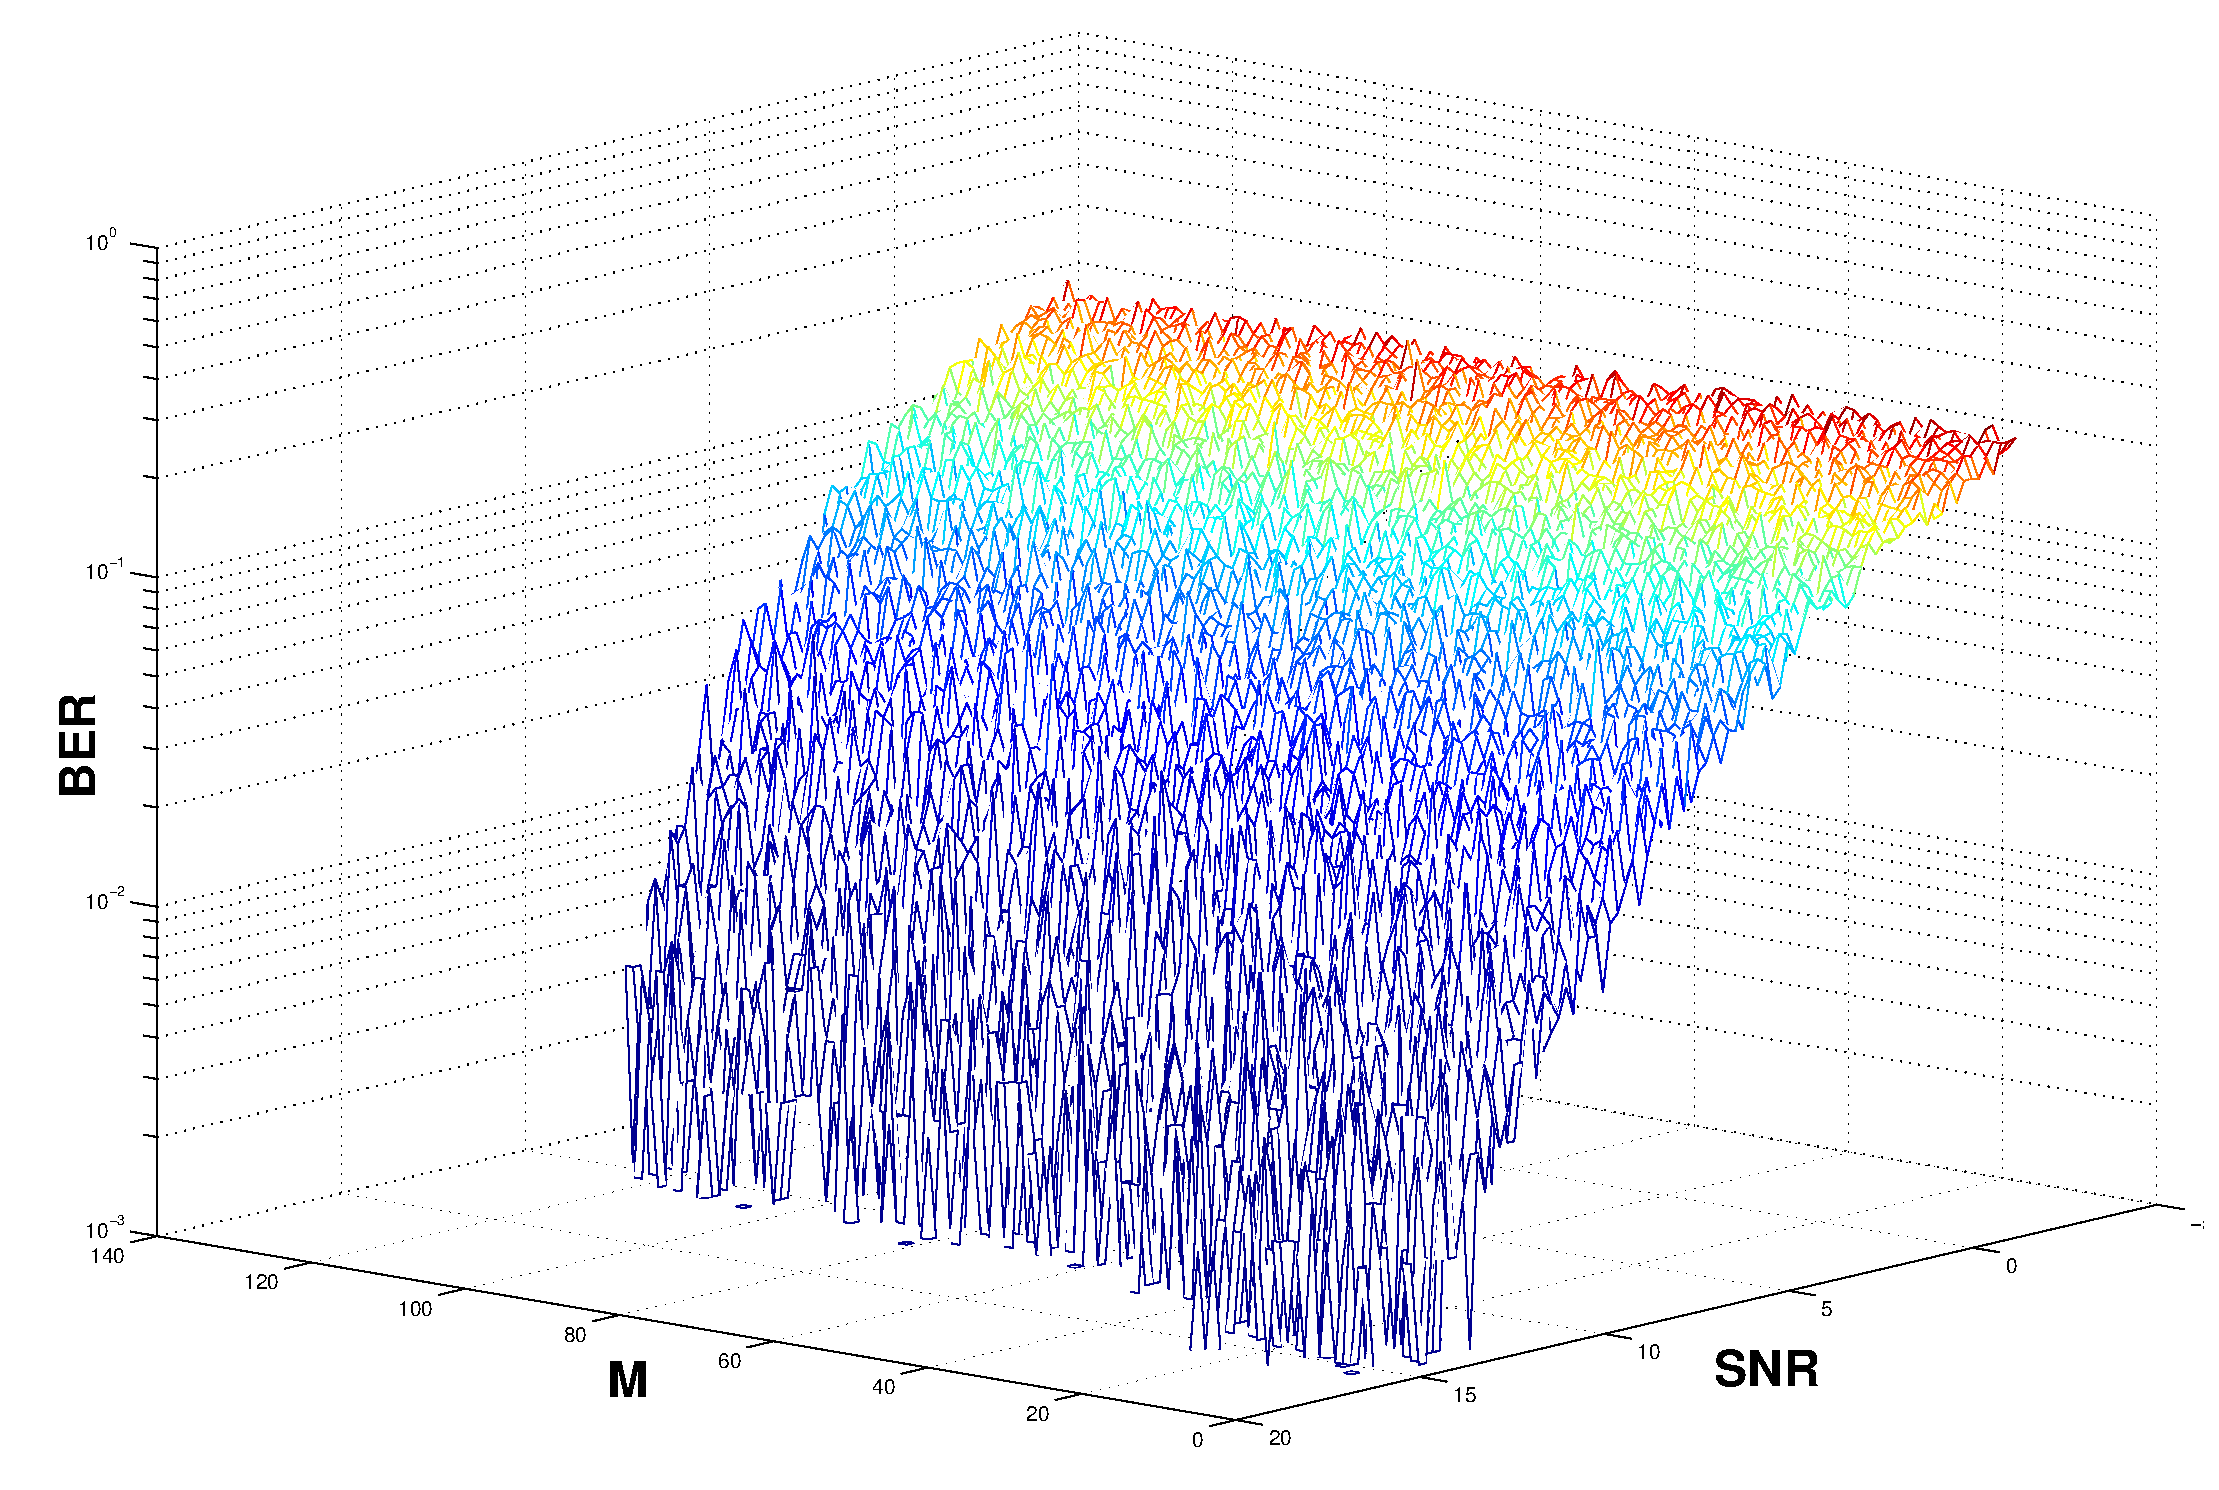
\includegraphics[width=2.5in]{BER_M_SNR_10_64_LSs.eps}
\caption{ The performance of the LS blind MUD against $M$ and
SNR.} }\label{BER_M_SNR}
\end{figure}
\section{Conclusions}
In this paper, we proposed a blind multiuser detection framework
as well as several blind detectors. The proposed blind detectors
are direct and simple without any channel or spreading sequence
estimation or subspace separation operation.
\small
\bibliographystyle{unsrt}
\bibliography{FastBDD}
\end{document}
